\section{Background}

	\subsection{Operating Systems Models}

		\begin{frame}[t]{Models of Operating Systems (OS)\\for Multicores}
		% \vspace{0.3cm}
		\begin{overprint}
			\only<1>{
				\begin{itemize}
					\item \textbf{Replicated OS}
					\item Master-Slave OS
					\item Symmetric OS
				\end{itemize}
				
				% \vspace{-0.3cm}

				\addfig[][width=.55\linewidth]{replicated-os.pdf}

				% \vspace{-0.3cm}

				\begin{center}
					Each core has a \textbf{copy of the OS}
				\end{center}
				\begin{center}
					\textbf{Less concurrency} but needs \textbf{a lot of memory}\\\textcolor{white}{abc}
				\end{center}
			}
			\only<2>{
				\begin{itemize}
					\item Replicated OS
					\item \textbf{Master-Slave OS}
					\item Symmetric OS
				\end{itemize}
				
				% \vspace{-0.3cm}

				\addfig[][width=.55\linewidth]{master-slave-os.pdf}

				% \vspace{-0.3cm}

				\begin{center}
					\textbf{Asymmetric execution} where only one core handles the OS
				\end{center}
				\begin{center}
					\textbf{Better scalability} and \textbf{less inter-core interference} but inserts a possible \textbf{bottleneck}
				\end{center}
			}
			\only<3>{
				\begin{itemize}
					\item Replicated OS
					\item Master-Slave OS
					\item \textbf{Symmetric OS}
				\end{itemize}
				
				% \vspace{-0.3cm}

				\addfig[][width=.55\linewidth]{symmetric-os.pdf}

				% \vspace{-0.3cm}

				\begin{center}
					\textbf{OS shared} by all cores
				\end{center}
				\begin{center}
					\textbf{Inter-core interference} and inefficient on processors without \textbf{cache coherence}
				\end{center}
			}
		\end{overprint}

			% Existem 3 modelos de sistema operacionais para multicores.
			% O primeiro, e mais simples, é o modelo replicado, onde cada núcleo possuem uma cópia distinta do SO. Isso elimina problemas de concorrência mas necessitando de muito espaço de memória.
			% Segundo, o modelo mestre-escravo define que apenas um único núcleo mestre lide com as estruturas do SO, e os escravos requisitem operações a ele. Também eliminando problemas de concorrência mas introduzindo um possível gargalo no sistema.
			% Terceiro, o modelo simétrico é o mais conhecido, ele permite o compartilhamento das estruturas internas forçando o uso de sincronização entre os núcleos do sistema. O que pode ser um problema para processadores que não possuem coerência de cache.
		\end{frame}

	\subsection{Message-Passsing Model}

		% \pholder[Software que lida com interfaces e dma?]{Low-Level Communication}
		\begin{frame}[fragile]{Low-Level Communication for\\Message-Passsing Model}
			\begin{itemize}
				\item \textbf{Computer network concepts}
			\end{itemize}

			\begin{itemize}
				\item Network interfaces
			\end{itemize}

			\begin{itemize}
				\item Performance impacts
				\begin{itemize}
					\item Number of intermediare copies
					\item Direct Memory Access (DMA)
				\end{itemize}
			\end{itemize}

			% Como Lightweight Manycores utilizam uma rede-em-chip para comunicação entre clusters,
			% a comunicação de baixo nível se assemelha a comunicação de uma rede de computadores.
			% Os nós da rede são conectados através de interfaces de rede.
			% O qual tem grande impacto na performace do sistema.
			% Por exemplo, a quantidade de cópias intermediárias ou no uso inadequado de DMAs podem afetar negativamente o desempenho.
		\end{frame}

		% \pholder[Tipos de envio/recebimento?]{User-Level Communication}
		\begin{frame}[fragile]{User-Level Communication for\\Message-Passsing Model}
		\begin{overprint}
			\only<1>{
				\begin{itemize}
					\item Send/receive primitives
					\begin{itemize}
						\item \textbf{Synchronous calls}
						\item Asynchronous calls
					\end{itemize}
				\end{itemize}

				\vspace{0.2cm}

				\addfig[][width=\linewidth]{call-sync.pdf}

				\begin{center}
					\textbf{Requester waits} for task to be completed
				\end{center}
			}
			\only<2>{
				\begin{itemize}
					\item Send/receive primitives
					\begin{itemize}
						\item Synchronous calls
						\item \textbf{Asynchronous calls}
					\end{itemize}
				\end{itemize}

				\vspace{0.2cm}

				\addfig[][width=\linewidth]{call-async.pdf}

				\begin{center}
					\textbf{Requester is released} to continue to run in parallel
				\end{center}
			}
		\end{overprint}

			% Utilizando os recursos de baixo nível, geralmente se exportam primitivas de envio ou recebimento de dados.
			% Essas primitivas podem implementar dois tipos de chamadas.
			% Chamadas síncronas força o requisitante a ficar bloqueado até que toda a operações for concluida.
			% Por outro lado, as chamadas assíncronas permitem que o requisitante continue sua executação após a configuração da primitiva. Isso permite que a síncronzação ocorra a posteriori.
		\end{frame}

	\subsection{Kalray MPPA-256}

		\begin{frame}[fragile]{Kalray MPPA-256}{A Lightweight Manycore Processor}

			\vspace{-0.45cm}

			\begin{columns}[totalwidth=\linewidth,t]
				\column{0.55\linewidth}

					\begin{itemize}
						\item \textbf{High-Performance and Low-Power Consunption}
					\end{itemize}

					\begin{itemize}
						\item \textbf{288 processing cores}
						\begin{itemize}
							\item {16 Compute Cluster (CC)}
							\item {4 I/O Cluster (IO)}
						\end{itemize}
					\end{itemize}

					\begin{itemize}
						\item \textbf{Data NoC (D-NoC)}
						\begin{itemize}
							\item 256 RX slots
							\item 8 TX channels
							\item 8 $\mu$threads for async TX
						\end{itemize}
					\end{itemize}

					\begin{itemize}
						\item \textbf{Control NoC (C-NoC)}
						\begin{itemize}
							\item 128 RX slots
							\item 4 TX channels
						\end{itemize}
					\end{itemize}

				\column{0.45\linewidth}
					\addfig[][width=.63\linewidth]{arch-mppa-2.pdf}
			\end{columns}

			% O processador MPPA-256 é um Lightweight Manycore de alto desempenho e baixo consumo energético.
			% Ele possui 288 núcleos de propósito geral agrupados em 16 clusters de computação e 4 clusters de entrada e saída.
		\end{frame}

		% \begin{frame}[fragile]{Kalray MPPA-256 Communication Resources}

		% 	% A comunicação é realizada através de duas NoCs distintas, uma para dados e outra para comandos.
		% 	% Cada NoC apresenta um conjunto de recursos para envio ou recebimento.
		% 	% Entretanto, a CNoC permite apenas a troca de mensagens de 64 bits.
		% \end{frame}

	\subsection{Nanvix OS}

		\begin{frame}[fragile]{The Nanvix Operating System}{Overview - The Nanvix Project}

		\begin{columns}[totalwidth=\linewidth]
		\column{.95\linewidth}

			% \vspace{1cm}

			\begin{columns}[totalwidth=\linewidth]
				\column{0.77\linewidth}

					\begin{itemize}
						\item \textbf{Open source} and \textbf{collaborative} project
						\begin{itemize}
							\item Home-grown instructional OS
							\item 4 Professors (Brazil and France)
							\item 1 PhD, 1 MSc and 3 BSc Students
							\item 9 past contributors
							\item UGA, PUC Minas, UFSC, and Grenoble INP
						\end{itemize}
					\end{itemize}

				\column{0.23\linewidth}
					\addfig[\tiny{\textit{Bingo, our mascot}}][width=\linewidth]{nanvix-logo.pdf}
			\end{columns} 


			% \vspace{.5cm}

			\begin{columns}[totalwidth=\linewidth]
				\column{0.6\linewidth}

					\begin{itemize}
						\item \textbf{Long-Term Goal}
						\begin{itemize}
							\item POSIX-Compliant OS
							\item Multikernel OS structure
							\item Asymmetric microkernels
							\item Flexible view of the plataform
						\end{itemize}
					\end{itemize}

				\column{0.4\linewidth}
					\addfig[][width=\linewidth]{nanvix-goal.pdf}
			\end{columns}

			% \vspace{1cm}

		\column{.1\linewidth}

			\begin{figure}
				\centering
				\begin{subfigure}
					
\includegraphics[width=.5\linewidth]{logo-gnu.png}
				\end{subfigure}%

				\vspace{.5cm}%

				\begin{subfigure}
					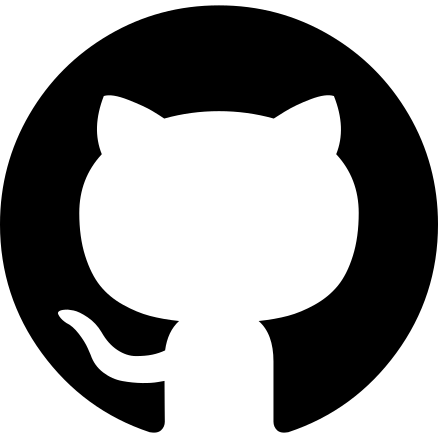
\includegraphics[width=.5\linewidth]{logo-github.pdf}
				\end{subfigure}%

				\vspace{.5cm}%

				\begin{subfigure}
					
\includegraphics[width=.5\linewidth]{logo-travis.png}
				\end{subfigure}%

				\vspace{.5cm}%

				\begin{subfigure}
					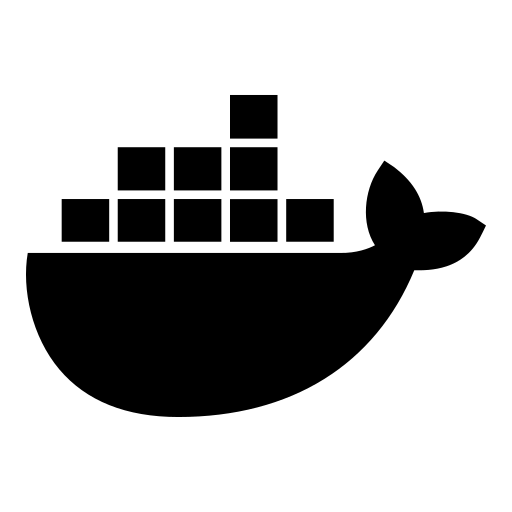
\includegraphics[width=.5\linewidth]{logo-docker.pdf}
				\end{subfigure}%
			\end{figure}

		\end{columns}
			% O Nanvix é um projeto de código aberto e colaborativo entre diversas universidades que busca fornecer melhor programabilidade e portabilidade para Lightweight Manycores através de um sistema compatível com o padrão POSIX.

			% Ele é subdivido em três níveis abstração, HAL, Microkernel e Multikernel.
		\end{frame}

		\begin{frame}[fragile]{Multikernel OS Structure}{Nanvix Multikernel Abstraction Layer}

			\begin{itemize}
				\item \textbf{OS services are system processes} and run in isolation
			\end{itemize}
			\begin{itemize}
				\item User processes \textbf{request services via message-passing}
			\end{itemize}

			\addfig[][width=.6\linewidth]{nanvix-multikernel-overview.pdf}

			% O Nanvix Multikernel, como o nome sugere, segue o modelo multikernel.
			% No qual os serviços do SO são processos que rodam isoladamente dos processos de usuário.
			% Assim, os processos de usuário requisitam serviços através da troca de mensagens.
		\end{frame}

		\begin{frame}[fragile]{Asymmetric Microkernel}{Nanvix Microkernel Abstraction Layer}

			\begin{itemize}
				\item Follows a \textbf{Master-Slave OS} model
				\item Provides \textbf{bare-bones of system abstractions}
				\item Rich system call interface (Kernel Call)
			\end{itemize}

			\addfig[][width=.6\linewidth]{nanvix-microkernel-overview.pdf}

			% O Nanvix Microkernel executa sobre a HAL e prove o esqueleto das abstrações do sistema.
			% Ele implementa o modelo Mestre-Escravo através de uma rica interface de chamadas de sistema.
			% Desta forma, ele é responsável por gerenciar os recursos da HAL e separar as reponsabilidades de mestre e escravo.
		\end{frame}

		\begin{frame}[fragile]{Flexible View of the Plataform}{Nanvix Hardware Abstraction Layer (HAL)}

			\begin{itemize}
				\item \textbf{Generic and flexible} hardware abstraction layer
				\item \textbf{Standard view} of these emerging processors
				\item Proposed interface within \textbf{Processador AL}
			\end{itemize}

			\addfig[][width=.6\linewidth]{nanvix-hal-overview.pdf}

			% A HAL é uma camada de abstração de hardware genérica e flexível.
			% Ela prove uma visão padronizada dos processadores.
			% Ela é composta por níveis que lidam com características de um único núcleo, entre os núcleos, e entre clusters.
			% Este trabalho está incluso na Camada de abstração do Processador, que envolve a interface de comunicação.
		\end{frame}

% LocalWords:  template cls standalone GitHub Overleaf bugfixes SVGs
% LocalWords:  Re-empacotamento fontsize Makefile pdflatex imgs PDFs
% LocalWords:  shell-escape frames SVG brazil english lapesd-slides
% LocalWords:  disabletodonotes todonotes TODO's backup showbackup
% LocalWords:  hidebackup abntexcite abntex natbib nobib titleframe
% LocalWords:  frame showsections sidebar stopcountingframes default
% LocalWords:  thanksframe Thank You Questions referencesframe titulo
% LocalWords:  bibfiles pholder todonote placeholder inline addfig
% LocalWords:  opts graphicx addfiglw width Citations dijkstra Direct
% LocalWords:  Closure Parallel dynamic scheduling DoImportantStuff
% LocalWords:  lccp merged cell svg pdf
